\documentclass[12pt]{article}
\usepackage{amssymb,amsmath, endnotes,setspace,enumerate,ulem,color,xspace,lscape,graphicx, cleveref}
\usepackage[sort]{natbib}
\allowdisplaybreaks[1]
\normalem
\newcommand{\textR}[1]{\textcolor{blue}{\texttt{#1}}}
\newcommand{\R}{\textR{R}}

\usepackage[none]{hyphenat}

\begin{document}

\title{Predicting Bitcoin returns and volatility with ARMA-GARCH models}

\author{
Kurt Ehlert \thanks{Department of Mathematics.  Email: {\tt kehlert@wisc.edu}}  % 1st author
\and 
August Jensen \thanks{Department of Statistics.  Email: {\tt  aljensen3@wisc.edu}}  % 2nd author
\and 
Bi Cheng Wu\thanks{Department of Statistics.  Email: {\tt  bwu62@wisc.edu}} % 3rd author
}

\maketitle

\begin{abstract}

% {\Huge

% \textbf{Q:} what do you call a bridge built by sexy gangsters?\\

% \textbf{A:} XXX G arch\\

% \textbf{Q:} how do models cope with psychological trauma?\\

% \textbf{A:} they auto-regress\\

% \textbf{Q:} how do you make a bland model taste better?\\

% \textbf{A:} add seasonality\\

% \textbf{Q:} why did the chicken cross the road?\\

% \textbf{A:} because through bootstrap forecasting it realized it's actually pretty unlikely to get hit by a car and so its generally pretty safe to cross the road.

% }

This paper explores the family of ARMA-GARCH models as a way to model financial data. The theory is discussed, showing how GARCH can capture properties such as volatility clustering, before moving on to a concrete example. The ARMA-GARCH model fitting process is demonstrated using daily log returns of Bitcoin closing prices. We found that a GARCH (1,1) model, without an ARMA component, is a reasonable model for the last year of log returns. Furthermore, we evaluated the model with bootstrapping techniques to obtain forecasts and prediction intervals. We conclude that a GARCH(1,1) model fails to explain some key aspects of the data such as extraordinarily heavy tails that cause bootstrapped standard errors to grow without bound.
\end{abstract}

\thispagestyle{empty}

\newpage
\pagenumbering{arabic} % add page numbers to your report

\section{Introduction}
\label{sec:introduction}

Financial data tends to have a lot of specific features associated with it. For example: there is often a trend and fluctuations of varying sizes, extreme values are more common, and volatility typically clusters. A standard ARMA model cannot account for properties such as those. Our motivation for this report was to try to find a model that better captures the distinctive features of financial data, and the approach we will explore here is the family of generalized auto-regressive conditional  heteroscedasticity (GARCH) models. First, we will discuss the underlying mechanisms behind the model that allow it to explain the properties above and more. Next, we will take a data set --- daily Bitcoin closing prices --- and put the theory in practice by fitting an ARMA-GARCH model on it, discussing the process as we go. Finally, we will evaluate the performance of our model and draw some conclusions.

\section{Theoretical Framework}
\label{sec:theory}
\subsection{Introduction}
In this section, we will present a brief overview of the theory relating to GARCH models in order to provide some context to the methods used in this report. Our aim is to give justification for applying the GARCH model to heteroscedastic data as we do with Bitcoin prices.

As mentioned earlier, time series for financial data tend not to be weakly stationary; there may be a trend over time, and it is common that the unconditional variance is non-constant. For instance, in the event of a market crash, volatility tends to be high as opposed to more stable times. We will see this type of behavior in our data set later on. In many cases, mean-stationarity can be restored by considering the log-return series---that is, if the original time series is denoted $X_t$, consider $\log(X_t/X_{t-1})$. From now on, we will consider a general mean-stationary series denoted by $Z_t$, which may be of this form for some series $X_t$. 

If $Z_t$ could be represented by an ARMA model, we assume that it is represented by the conditional expectation of the series at time $t$ plus a prediction error term, where we condition on past knowledge up to time $t-1$. To borrow the notation from Box \& Jenkins (361), let $F_{t-1} = \{Z_s | s<t \}$ be the past knowledge and $a_t = \epsilon_t$ be the innovation. \cite{box} Then, we have for an ARMA model $\phi(B)Z_t = \delta + \theta(B)a_t$, $$Z_t = E[Z_t|F_{t-1}] + a_t$$ where the $a_t$ are assumed to be independent and homoscedastic with variance $\sigma^2_a$. However, as we will demonstrate later, these independence and homoscedasticity assumptions often fail to hold in the data we are interested in.  Other problematic features of financial data that are not covered by ARMA models include: asymmetrical responses, heaviness of the tails of the marginal distribution of $Z_t$ (allowing for more ``extreme'' values), volatility clustering (periods over which volatilities are similar), and serial dependence with zero correlation.

\subsection{ARCH models}
\subsubsection{Definition of ARCH(s)}

Our first step is to introduce the class of autoregressive conditional heteroscedasticity models, abbreviated as ARCH models. For $e_t \sim \text{IID}(0,1)$, the ARCH(s) model is 
\begin{equation}
    a_t = \sigma_t e_t
\end{equation}
\begin{equation}
    \sigma_t^2 = \alpha_0 + \sum_{j=1}^{s} \alpha_ja^2_{t-j}
\end{equation}
We assume that $\alpha_0 > 0$, $\alpha_s > 0$, and the coefficients all are non-negative. This guarantees that $\sigma^2_t > 0$ for every integer $t$. Furthermore, to guarantee weak stationarity and existence of the variance of $a_t$, we also set $\sum_{j=1}^{s} \alpha_j < 1$. Recall that we mentioned the heavy-tailed behavior of financial data: to accommodate this, we often set the distribution of the $e_t$ terms to be a Student's t-distribution. 

\subsubsection{Properties of ARCH(1)}

It is illustrative to begin with ARCH(1) and develop properties of interest that can then be generalized to ARCH(s). We start with the following basic properties:

\begin{enumerate}
    \item $\sigma^2_t =$ Var$[a_t|F_{t-1}] = E[a^2_t|F_{t-1}] = \alpha_0 + \alpha_1a^2_{t-1}$
    
    \item $E[a_t] = 0$
    
    \item $E[a_ta_{t-j}] = 0$ for $j>0$
    
    \item The $a_t$ are not mutually independent
    
\end{enumerate}


Now, we will prove the above statements. 


\begin{itemize}

    \item \textbf{Property 1}: We have that $a_t = \sigma_t e_t$ where $\sigma^2_t = \alpha_0 + \alpha_1 a^2_{t-1}$. Recall that $F_{t-1}$ represents past information and $\sigma^2_t$ depends solely on past information ($a^2_{t-1}$), so we have that $$E[a_t|F_{t-1}] = E[\sigma_t e_t | F_{t-1}] = \sigma_t E[e_t|F_{t-1}] = 0$$ by independence of the innovations. 

    \item \textbf{Property 2}: This is a direct consequence of Property 1: consider $E[E[a_t|F_{t-1}]]$.

    \item \textbf{Property 3}: We use the tricks from the above two proofs: we have that $$E[a_ta_{t-j}] = E[E[a_ta_{t-j}|F_{t-1}]] = E[a_{t-j}E[a_t|F_{t-1}]] = 0$$  Note that we assume that $j>0$, so the past information includes $a_{t-j}$.
    
    \item \textbf{Property 4}: The definition of $\sigma^2_t =$ Var($a_t|F_t$) shows that the $a_t$ are not mutually independent.

\end{itemize}

\indent Notice that Property 3 implies that the $a_t$ are uncorrelated. This is crucial for the efficient market hypothesis, which postulates that asset prices reflect all current available information.  Property 1 helps us find the unconditional variance of $a_t$: consider $$Var[a_t] = E[a^2_t] = E[E[a^2_t|F_{t-1}] = E[\alpha_0 + \alpha_1a^2_{t-1}] = \alpha_0 + \alpha_1\sigma^2_a$$ Therefore, we have:  
    \begin{equation}
    \sigma^2_a = Var[a_t] = \frac{\alpha_0}{1-\alpha_1}
    \end{equation}
    
    This is why we required that the sum of the coefficients be less than 1; it guarantees that the variance exists. To conclude this section, define $\nu_t = a^2_t - \sigma^2_t$ and notice that 
    \begin{equation}
        a^2_t = \alpha_0 + \alpha_1a^2_{t-1} + \nu_t
    \end{equation}
    
    We have that $E[\nu_t] = 0$ by definition and  that the $\nu_t$ are uncorrelated. Thus, this defines an AR(1) model for $a_t$ that is weakly stationary. This shows that the ARCH(1) model is equivalent to an AR(1) model on the squared error term in some ARMA model. However, note that the $\nu_t$ are not homoscedastic. 



\subsubsection{Generalizing to ARCH(s)}

It is straightforward to generalize the last result above to ARCH(s). Define $\nu_t$ in the same way as before. Now, we have: 
    \begin{equation}
        a^2_t = \alpha_0 + \sum_{j=1}^{s} \alpha_ja^2_{t-j} + \nu_t
    \end{equation}

This is clearly an AR(s) model for $a^2_t$. The results for ARCH(1) generalize easily; as $F_{t-1}$ includes past information, the proofs are largely unchanged. One thing to note is that we now have 
    \begin{equation}
        \sigma^2_a = \frac{\alpha_0}{1-\sum_{j=1}^{s} \alpha_j}
    \end{equation}

As in the ARCH(1) case, we see why the assumption of $\sum_{j=1}^{s} \alpha_j < 1$ is necessary. 

\subsubsection{Forecasting}

Baillie and Bollerslev showed that, for an ARMA model on $Z_t$ with independent and identically distributed $a_t$, heteroscedasticity does not affect the minimum mean-square error forecasts \cite{baillie}. In other words, this tells us that we can forecast the conditional mean as usual while forecasting the volatility using our ARCH(s) model. However, the variance of the forecasts will be affected, so prediction intervals won't be the same.

\subsection{GARCH Models}

Now, let us generalize the previous section: we showed that an ARCH(s) model was equivalent to an AR(s) model on the squared error terms. What if we now allowed that there be a MA component? The GARCH(s,r) model is given as:
    \begin{equation}
        a_t = \sigma_t e_t
    \end{equation}
    \begin{equation}
        \sigma_t^2 = \alpha_0 + \sum_{j=1}^{s} \alpha_ja^2_{t-j} + \sum_{j=1}^{r} \beta_j \sigma^2_{t-j}
    \end{equation}
We have the assumptions that $\alpha_0 > 0$, $\alpha_s > 0$, $\beta_r > 0$, and the coefficients all are non-negative. To guarantee the existence of the unconditional variance, we impose the following condition: $\sum_{j=1}^{max(s,r)} (\alpha_j + \beta_j) < 1$. We also usually set the error distribution to be something like a Student's t-distribution as with ARCH(s). The results from the previous section generalize for GARCH(s,r) models, so we will only list the main points. Note that (9) tells us that we have an ARMA(max(s,r),r) model on the squared error terms given the same definition for $\nu_j$ as before. 

\begin{equation}
    a^2_t = \alpha_0 + \sum_{j=1}^{max(s,r)} (\alpha_j + \beta_j)a^2_{t-j} +  \nu_t - \sum_{j=1}^{r} \beta_j\nu_{t-j}    
\end{equation}
\begin{equation}
    \sigma^2_a = Var(a_t) = \frac{\alpha_0}{1-\sum_{j=1}^{max(s,r)} (\alpha_j + \beta_j)}
\end{equation}

 GARCH(1,1) is the most common model used; it is rare to see orders higher than 1. The following properties carry over from ARCH(s):

\begin{enumerate}
    \item $\sigma^2_t =$ Var$[a_t|F_{t-1}] = E[a^2_t|F_{t-1}] = \alpha_0 + \alpha_1a^2_{t-1} + \beta_1\sigma^2_{t-1}$
    
    \item $E[a_t] = 0$
    
    \item $E[a_ta_{t-j}] = 0$ for $j>0$
    
    \item The $a_t$ are not mutually independent
    
\end{enumerate}

The proofs are identical to the ARCH(1) case, so we are able to easily generalize these results to the GARCH(s,r) case. As we discussed earlier, we can see why GARCH models are attractive regarding financial data. First, we can account for heavy-tail behavior by setting the error distribution to be heavy-tailed. Second, volatility clustering occurs naturally within our model---observe that if $a^2_{t-1}$ or $\sigma^2_{t-1}$ are large, $\sigma^2_t$ tends to be as well and similarly for small values. Also, dependence without correlation is clear from Properties 3 and 4. Another nice property of GARCH is apparent when dealing with parameter estimation using conditional maximum likelihood. Quoting from Box and Jenkins, ``the information matrix of the log-likelihood is block diagonal with respect to the conditional mean and variance parameters, so that iterations can be carried out separately with respect to the two sets of parameters.'' (369) \cite{box} However, GARCH does not capture all of the properties found in financial data. In the model, the conditional mean is unaffected by volatility so there is no ``risk premiums''. Also the leverage effect (negative correlation between changes in volatility and changes in returns) is unaccounted for, and furthermore some issues can arise with high-frequency data about near-unit roots. There are modified models that attempt to deal with these issues, such as EGARCH, shown here
\begin{equation}
    ln(\sigma^2_t) = \alpha_0 + g(e_{t-1}) + \beta_1 ln(\sigma^2_t)
    \end{equation}
\begin{equation}
    g(e_{t-1}) = \alpha_1 e_{t-1} + \gamma_1 |e_{t-1}| - \gamma_1 E[|e_{t-1}|]
\end{equation}
EGARCH accounts for leverage effects by allowing for asymmetrical responses: a positive shock has effect $(\alpha_1 + \gamma_1)e_{t-1}$ and a negative one has effect $(\alpha_1 - \gamma_1)e_{t-1}$. If leverage is present, $\alpha_1 < 0$. We will fit an EGARCH model later on to demonstrate, but we will leave out discussion about other modified GARCH models as the focus of this paper is primarily on the base GARCH model.

\section{Statistical analysis}
Bitcoin is an ``alternative currency'' that has recently exploded in popularity. Concomitant with its popularity, its price has fluctuated wildly. In fact, its price has crashed by over 80\% since last year. We decided to analyze the log-returns of Bitcoin at a daily level. Since the Bitcoin exchanges do not close unlike, for example, the New York Stock Exchange, there is not a natural choice for a daily closing price. Thus we arbitrarily chose to call the midprice at 7 PM EST the ``daily closing price''.

The top of \Cref{fig:log_ret} shows the log-returns over the past five years, and the bottom plot shows them over the last year. We can see that the volatility fluctuates dramatically over the past five years and it clusters. Also, there are many days with extreme positive or negative log-returns. All of those phenomena are typical of financial time series data. An ARMA model cannot capture such changes in volatility, so we attempted to fit an ARMA-GARCH model.

\begin{figure}
    \centering
    \includegraphics[width=\textwidth]{log_ret.pdf}
    \caption{Daily log returns from holding Bitcoin. A trading day is defined as starting at 7 PM EST and ending 24 hours later.}
    \label{fig:log_ret}
\end{figure}

First we applied the augmented Dickey-Fuller test to test for stationarity. The p-values were all around 0.01, which is strong evidence that the series is stationary. But we should note that heteroscedasticity may invalidate the results of the test. Nevertheless, we take the results as an indicator that we may proceed with fitting an ARMA model to explain the conditional mean.

The ACF and PACF of the log-returns are hard to interpret. By that we mean it is not immediately clear which ARMA model, if any, is appropriate for the time series. If an ARMA model cannot satisfactorily capture the behavior of the conditional mean, it would not be too surprising. The price dynamics of Bitcoin likely depend on a wide variety of factors that are not accounted for in an ARMA model. We will discuss this further later on.

We can also see that the ACF of the squared log-returns decays slowly, which is typical of a heteroscedastic time series (\Cref{fig:log_ret_acfs}). To put it simply, the conditional variance depends on the previous variance and/or innovations. We already suspected that a GARCH model would be appropriate for this data, and the slow decay of the ACF further confirms our hypothesis.

\begin{figure}[h]
    \centering
    \includegraphics[width=0.75\textwidth]{log_ret_acfs.pdf}
    \caption{Shown are the (partial) autocorrelation functions of the five years worth of Bitcoin daily log-returns.}
    \label{fig:log_ret_acfs}
\end{figure}

We attempted to fit various ARMA models to the data, however they did not have much success. In particular, we focused on an MA(11) model. After fitting the model with R, we computed p-values for testing whether or not the coefficients were significantly different from zero. The p-values of the coefficients assumed normality. Technically a t-distribution would be more appropriate, but we have enough time points to feel comfortable just using the normal p-values.

We then found a more parsimonious model by dropping the coefficients with p-values greater than 0.05 one-by-one. After dropping each coefficient, we fit the model again and repeated the process. We ended up with an MA(11) model where only the coefficients corresponding to the lags at 5, 6, 10, and 11 were nonzero. We then ran the Box-Ljung test on the residuals.

For lags less than 26, the p-values were greater than 0.05, which indicates that the residuals are likely white noise. However, for larger lags the p-values approached 0.01. Typically we would conclude that the MA model is not a good fit, but before tossing out the model, we decided to start fitting a GARCH component. Perhaps the Box-Ljung p-values were small due to heteroscedasticity. We also tried fitting models with an AR component, but the MA models were at least as successful. 

We fit an MA(11)-GARCH(2,2) model to the data, with the appropriate MA coefficients set to zero. The errors were taken to be t-distributed, since the normal distribution did not capture the shape of the fat-tailed errors (\Cref{fig:garch_22_residuals}). R computed the p-values of the coefficients, and many of them were well above 0.05. Therefore, just like before, we set the least significant coefficients to zero, and then refit the model. The process was repeated until all of the coefficients were significant (p-value less than 0.05). We ended up with an MA(6)-GARCH(1,1) model. \Cref{tab:garch_22_coeffs} shows the coefficients and their corresponding statistics.

\begin{figure}[h]
    \centering
    \includegraphics[width=0.5\textwidth]{garch_22_residuals.pdf}
    \caption{Empirical and fitted distributions of the standardized residuals after fitting an MA(11)-GARCH(2,2) model. The t-distribution does a much better job of capturing the shape of the empirical distribution.}
    \label{fig:garch_22_residuals}
\end{figure}

\begin{table}[h!]
\begin{center}
\begin{tabular}{|l | l | l | l | l | l | l | l | l | l | l |}
\hline
Coefficient & Estimate & Robust Std. Error & t value & p value\\
mu     & 0.0015 & 0.00046 & 3.18 & 0.0015\\
ma6 & 0.060 & 0.020 & 3.019 & 0.0025\\
alpha1 & 0.11 & 0.014 & 7.41 & 0\\
beta1  & 0.89 & 0.17 & 53.58 & 0\\
shape & 3.59 & 0.17 & 21.00 & 0\\
\hline
\end{tabular}
\end{center}
\caption{Coefficient information of the MA(6)-GARCH(1,1) model fitted to five years worth of data.}
\label{tab:garch_22_coeffs}
\end{table}


We also plotted the conditional mean plus/minus two standard deviations from the GARCH model, and then overlaid the actual log-returns (\Cref{fig:garch_five_year_fit}). The QQ plot suggests that the t-distributions fits the actual errors fairly well, however the tails of the actual errors are still larger than what the t-distribution predicts. Some of the days had huge sudden up or down price moves, which is probably why the tails do not match up.

In order to assess our model, we examined the ACF and the standardized residuals and their squares. R also computed the Box-Ljung p-values. The p-values for the standardized residuals were essentially 0, so the conditional mean is not explained well by our model. However, the p-values for the standardized squared residuals were all above 0.4. Therefore, we should reject the null hypothesis that the standardized residuals are white noise, but accept that their squares are white noise. In conclusion, the GARCH(1,1) model seems to explain the conditional variance but the MA(6) model does not help explain the conditional mean.

\begin{figure}[h]
    \centering
    \includegraphics[width=0.8\textwidth]{garch_five_year_fit.pdf}
    \caption{Various plots for assessing the fit of the MA(6)-GARCH(1,1) model with the insignificant coefficients set to 0. See \Cref{tab:garch_22_coeffs} for information on the coefficients.}
    \label{fig:garch_five_year_fit}
\end{figure}

If we look again at the data, we see that price quickly crashed or rose within some of the days. The extreme price movements may have prevented us from finding a satisfactory ARMA model. Furthermore, the market conditions of Bitcoin have changed substantially over the last five years. It has gotten a lot more media attention and more money has flowed into the currency, especially in the last two years. In fact, the Chicago Mercantile Exchange launched Bitcoin futures contracts in December of 2017. The point of mentioning all this is to argue that since the Bitcoin market has changed so dramatically within the last two to three years, trying to fit the last five or so years of data might be too ambitious. Even if we can fit the data, we are essentially averaging over drastically different market conditions, which might be less useful than fitting a model to only more recent data.

If we accept that conclusion, then it makes sense to fit data from just the last year. The ACF indicates that an ARMA model is unnecessary for explain the conditional mean (\Cref{fig:acf_one_year}). To be rigorous, we also computed all of the Box-Ljung test p-values ranging from lag 1 to 10, and the p-values were at least 0.1, and were usually much higher. Therefore a constant conditional mean might be an appropriate choice.

\begin{figure}[ht]
    \centering
    \includegraphics[width=0.5\textwidth]{acf_one_year.pdf}
    \caption{ACF of the daily log-returns over the last year.}
    \label{fig:acf_one_year}
\end{figure}

We then went through the same process as described earlier to fit a GARCH model. The errors were assumed to follow a skewed t-distribution. \Cref{fig:one_year_residuals} shows that the normal distribution does not have fat enough tails, and the regular t-distribution did not capture the apparent positive skew of the errors. We started with a GARCH(2,2) model and ended up with a GARCH(1,1) model with a conditional mean equal to zero. \Cref{tab:garch_one_year_coeffs} shows the coefficient information. If we ignore the single large spike, the ACF of the standardized residuals and their squares look like that of white noise (\Cref{fig:garch_one_year_fit}), and the QQ plot indicates that the skewed t-distribution does a reasonable job. However, the tails are still not entirely explained by the model.

\begin{figure}[h!]
    \centering
    \includegraphics[width=0.75\textwidth]{one_year_residuals.pdf}
    \caption{Empirical and fitted distributions of the standardized residuals after fitting a GARCH(1,1) model to the last year of data. Compared to the normal or standard t-distributions, the skewed t-distribution does a much better job of capturing the shape of the empirical distribution.}
    \label{fig:one_year_residuals}
\end{figure}

\begin{table}[h!]
\begin{center}
\begin{tabular}{|l | l | l | l | l | l | l | l | l | l | l |}
\hline
Coefficient & Estimate & Robust Std. Error & t value & p value\\\hline
alpha1 & 0.0738 & 0.019 & 3.85 & 0\\
beta1  & 0.925 & 0.016 & 58.87 & 0\\
skew & 0.90 & 0.50 & 18.31 & 0\\
shape & 3.93 & 0.60 & 6.49 & 0\\
\hline
\end{tabular}
\caption{Coefficient information of the GARCH(1,1) model fitted to data from the last year.}
\label{tab:garch_one_year_coeffs}
\end{center}
\end{table}

\clearpage

Despite the large spike in the ACF, the The Box-Ljung p-values for the standardized residuals and their squares are well above 0.1 up to at least lag 10. Thus the GARCH(1,1) model with a constant conditional mean fits the data quite well. Actually, the large spike at lag five is due to the price of Bitcoin crashing dramatically in the last couple of weeks. If we remove the last two weeks of data, then the large spike in the ACF goes away and also the QQ plots look much better.

\begin{figure}[h!]
    \centering
    \includegraphics[width=0.8\textwidth]{garch_one_year_fit.pdf}
    \caption{Various plots for assessing the fit of the GARCH(1,1) model with the insignificant coefficients set to 0. The model was fitted to the last year of data. See \Cref{tab:garch_one_year_coeffs} for information on the coefficients.}
    \label{fig:garch_one_year_fit}
\end{figure}

The standard GARCH model that we used does not allow for asymmetric reactions to positive and negative returns. However, exponential GARCH (EGARCH) does allow for exactly that. We fit EGARCH(2,2) to the last year of data. The QQ plot suggests that the extreme downward events are better captured by the EGARCH model compared to the GARCH model. Also, the ACF of the standardized squared residuals looks better (\Cref{fig:egarch_one_year_fit}). The large spike is less significant, which also coincides with the hypothesis that the EGARCH model does a better job of dealing with extreme events. Arguably, the fits of the GARCH and EGARCH models are not drastically different, so one might prefer the simpler GARCH(1,1) model.

\begin{figure}[h]
    \centering
    \caption{Various plots for assessing the fit of the EGARCH(1,1) model with the insignificant coefficients set to 0. The model was fitted to the last year of data. The coefficients $\omega$ and $\mu$ were set to zero.}
    \includegraphics[width=0.8\textwidth]{egarch_one_year_fit.pdf}
    \label{fig:egarch_one_year_fit}
\end{figure}

\clearpage

\section{Model Performance}

\subsection{Method}

To evaluate the performance of our model, a bootstrap-based technique propose by Pascual, Rorno, \& Ruiz (2004) was chosen \cite{pascual}.

To summarize the method, first the residuals from the fitted model are centered and rescaled. Then, from this empirical distribution new residuals are sampled independently and used in the model equation to construct alternate realizations of the time series. The model equation is then refitted and the coefficients and forecasts of each iteration recorded. This process is repeated $B$ times and the resulting distributions of coefficients and predicted values can be used to construct approximate confidence intervals.

The main advantage of this method is the ability to capture the variation of the fitted models' coefficients, which are typically not easily solvable and often presumed to be constant once the best model has been fitted. It also doesn't assume Gaussian innovations, unlike the more traditional method by Box \& Jenkins \cite{box}.

Other attempts at developing bootstrap methods have been proposed before (see \cite{pascual} for a more detailed discussion of alternative methods) but this method was chosen both for its minimal assumptions and simplicity of implementation. It has also been shown to outperform most alternatives in simulation studies \cite{pascual}.

\subsection{Results}

Two of the final candidate GARCH(1,1) models were compared: one fitted with all Bitcoin data we have going back to 2013 with $\omega$ fixed to be $0$, and the other with only recent data from the past year with $\mu,\omega$ both fixed to $0$, since both were deemed insignificant. The \texttt{ugarchboot} function in package \texttt{rugarch} provides a fast multithreaded implementation of Pascual's bootstrap method. The forecast range was set to 6-months, or 2 quarters to test for long-term stability of predictions. 1000 bootstrap iterations were performed.

\Cref{fig:params} shows the resulting  distribution of fitted model coefficients. Note the model fitted with only recent (past-year) data fixes $\mu=0$ due to being dropped for lack of significance whereas the $\mu$ is significant in the complete-data model. It is interesting to note that model parameters fixed to be $0$ in the fit result in an almost perfectly Gaussian distribution around the fixed value $0$ in the bootstrapped coefficients. Other coefficients which are not fixed have much more erratic distributions, and are often heavily skewed and even bimodal. These variations are all easily captured in the bootstrapped forecasting and confidence intervals, which are presented in \Cref{fig:cast}.

In \Cref{fig:cast}, the red line shows the naive 1-step ahead forecasts, the black line shows the bootstrapped forecast by sampling residuals, and the 4 lines formed by numerous dots represent respectively $5\%$, $25\%$, $75\%$, and $95\%$ quantiles for the bootstrapped forecasts.

\subsection{Discussion and Conclusion}

Both models performed reasonably for the first quarter (90 days); the bootstrapped predictions generally fall reasonably well within the bounds, but beyond that, the all-data model becomes very chaotic and seems to diverge beyond expected bootstrapped confidence interval bounds whereas the recent-data model seems slightly more stable.

Additionally, in the all-data models, note the increased deviation of the bootstrapped residual standard errors from expected bounds starting just around 1 quarter in the future, whereas the recent-data model respects the bounds fairly well. This seems to indicate that the data older than a year may have significant deviation from the theoretical model, which causes the ARMA residuals to increase at a faster rate than GARCH predicts. In other words, there may be additional sources of heteroscedasticity that are as yet unaccounted for by the model. This may be a major contributing factor to the long-term extreme volatility of the time series forecasts for this model.

As a final point, it is interesting to note that in both models, the $95\%$ interval upper bound for residual error increases steadily over time while the $25\%$ upper bound is fairly steady. This was an unexpected discovery and seems to imply that although the majority of bootstrapped time series show fairly predictable changes in variance over time, the tails of the residual standard error become heavier over time and it becomes increasingly likely to observe extreme outlier-like observations, even in the fairly well-behaved recent-data model, where the heteroscedasticity in the data is well explained by the fitted model.

In conclusion, it seems that short-term fluctuations in Bitcoin closing prices (with the exception of sudden shocks due to pressures external to the market) are fairly well modelled using a simple GARCH(1,1) model; however, long-term forecasts of prices past 1 quarter are likely to be untrustworthy and highly prone to error due to the inherent volatility of the underlying asset price.

\begin{figure}[h]
\begin{center}
\centering
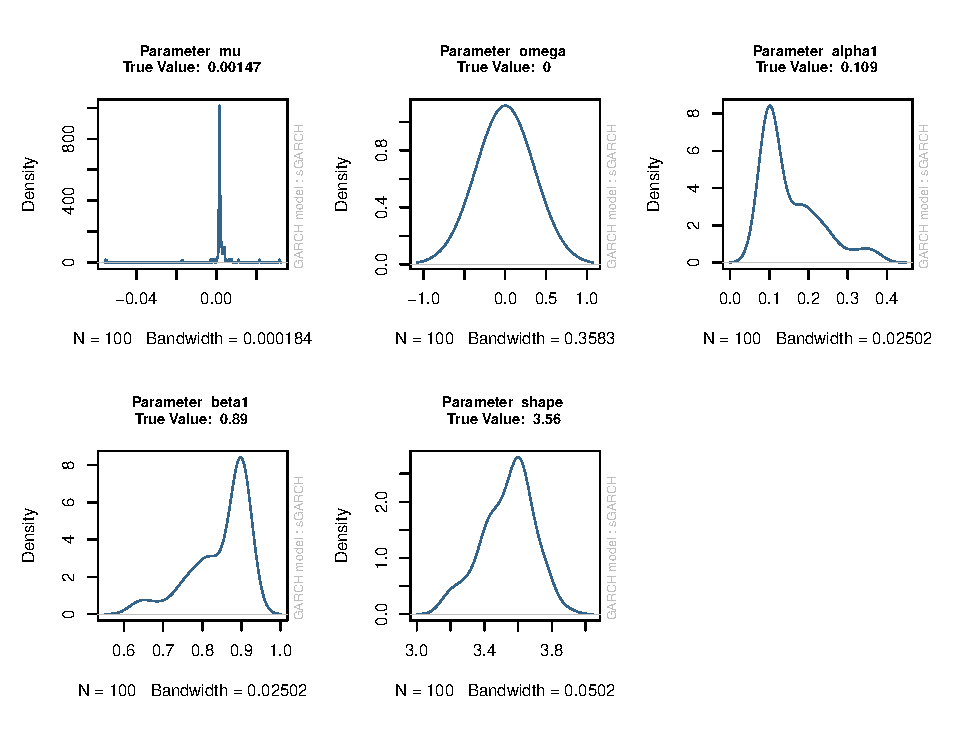
\includegraphics[width=.8\linewidth,height=.46\linewidth,trim={0 -20 0 0}]{boot_param_all}\\
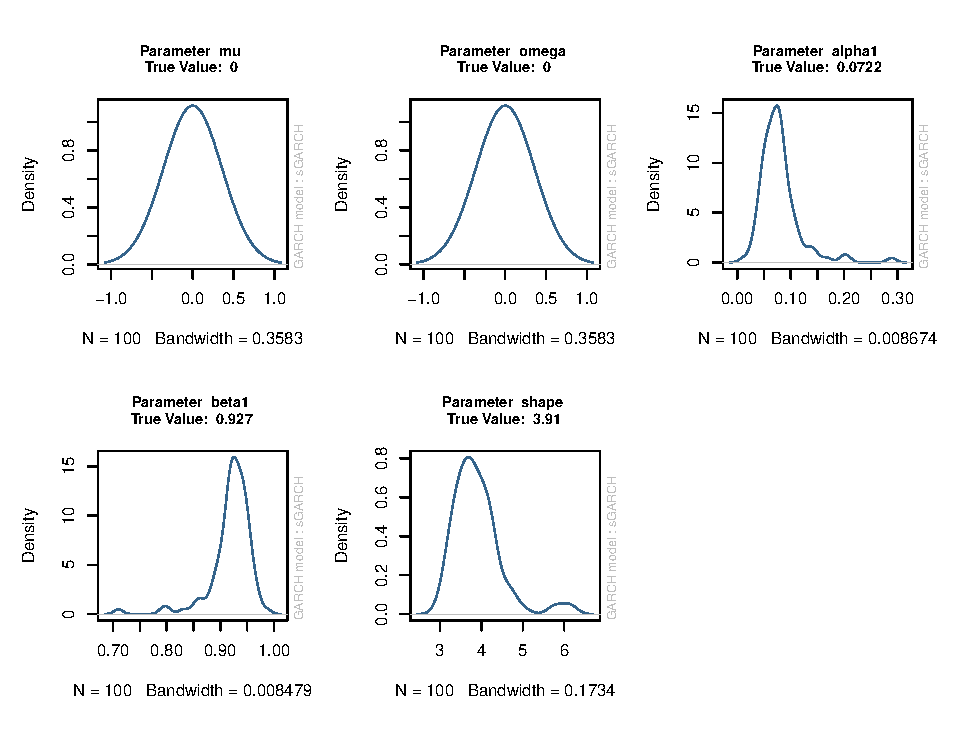
\includegraphics[width=.8\linewidth,height=.46\linewidth]{boot_param_recent}\\
\caption{Parameter distributions for fitted models. Top five plots are for all data; bottom five plots are for recent (past-year) data.}
\label{fig:params}
\end{center}
\end{figure}

\begin{figure}[h]
\begin{center}
\centering
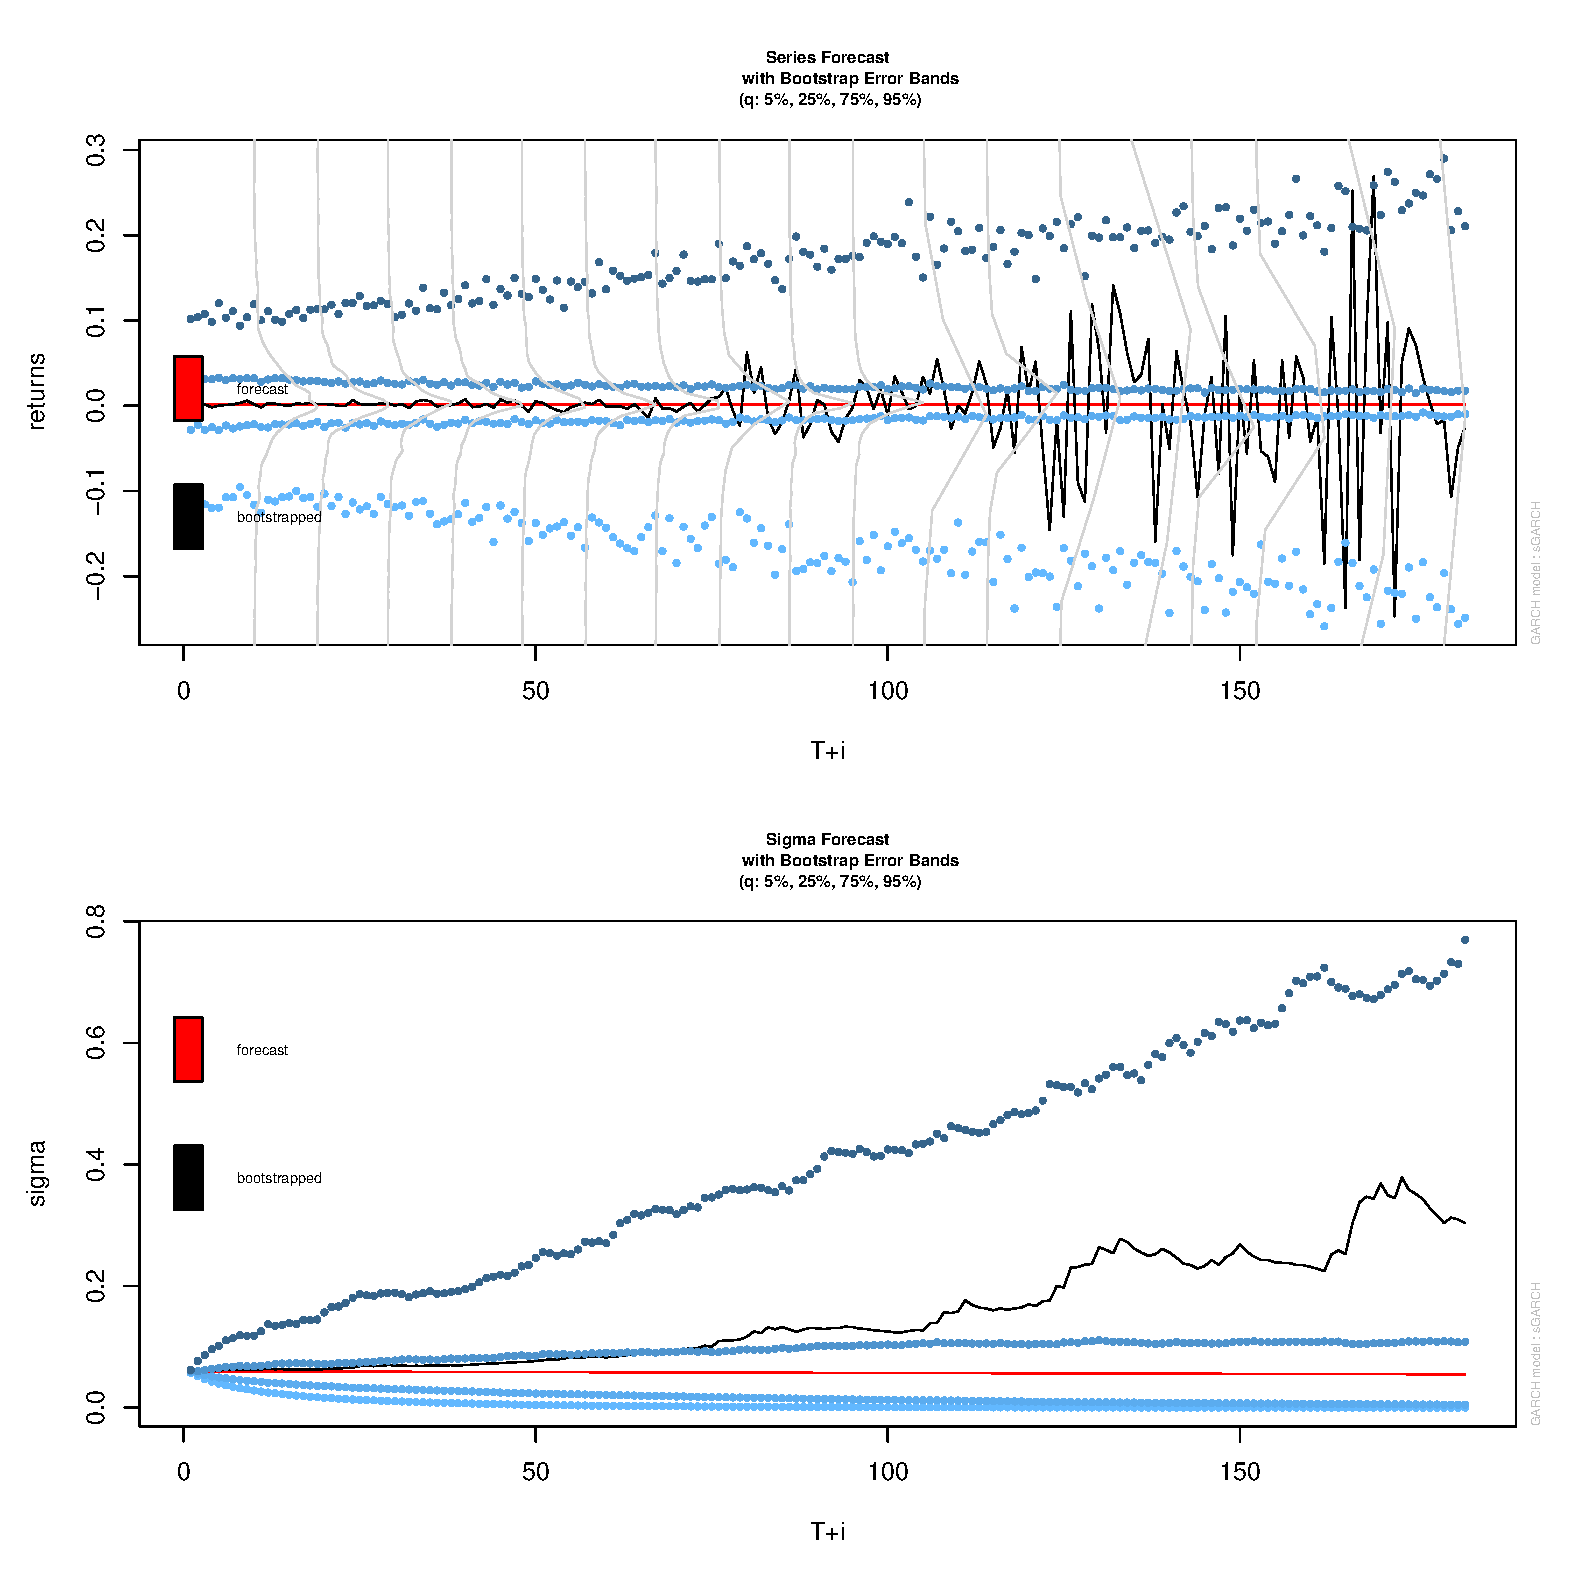
\includegraphics[width=.9\linewidth,height=.65\linewidth,trim={0 -50 0 125}]{boot_cast_all}\\
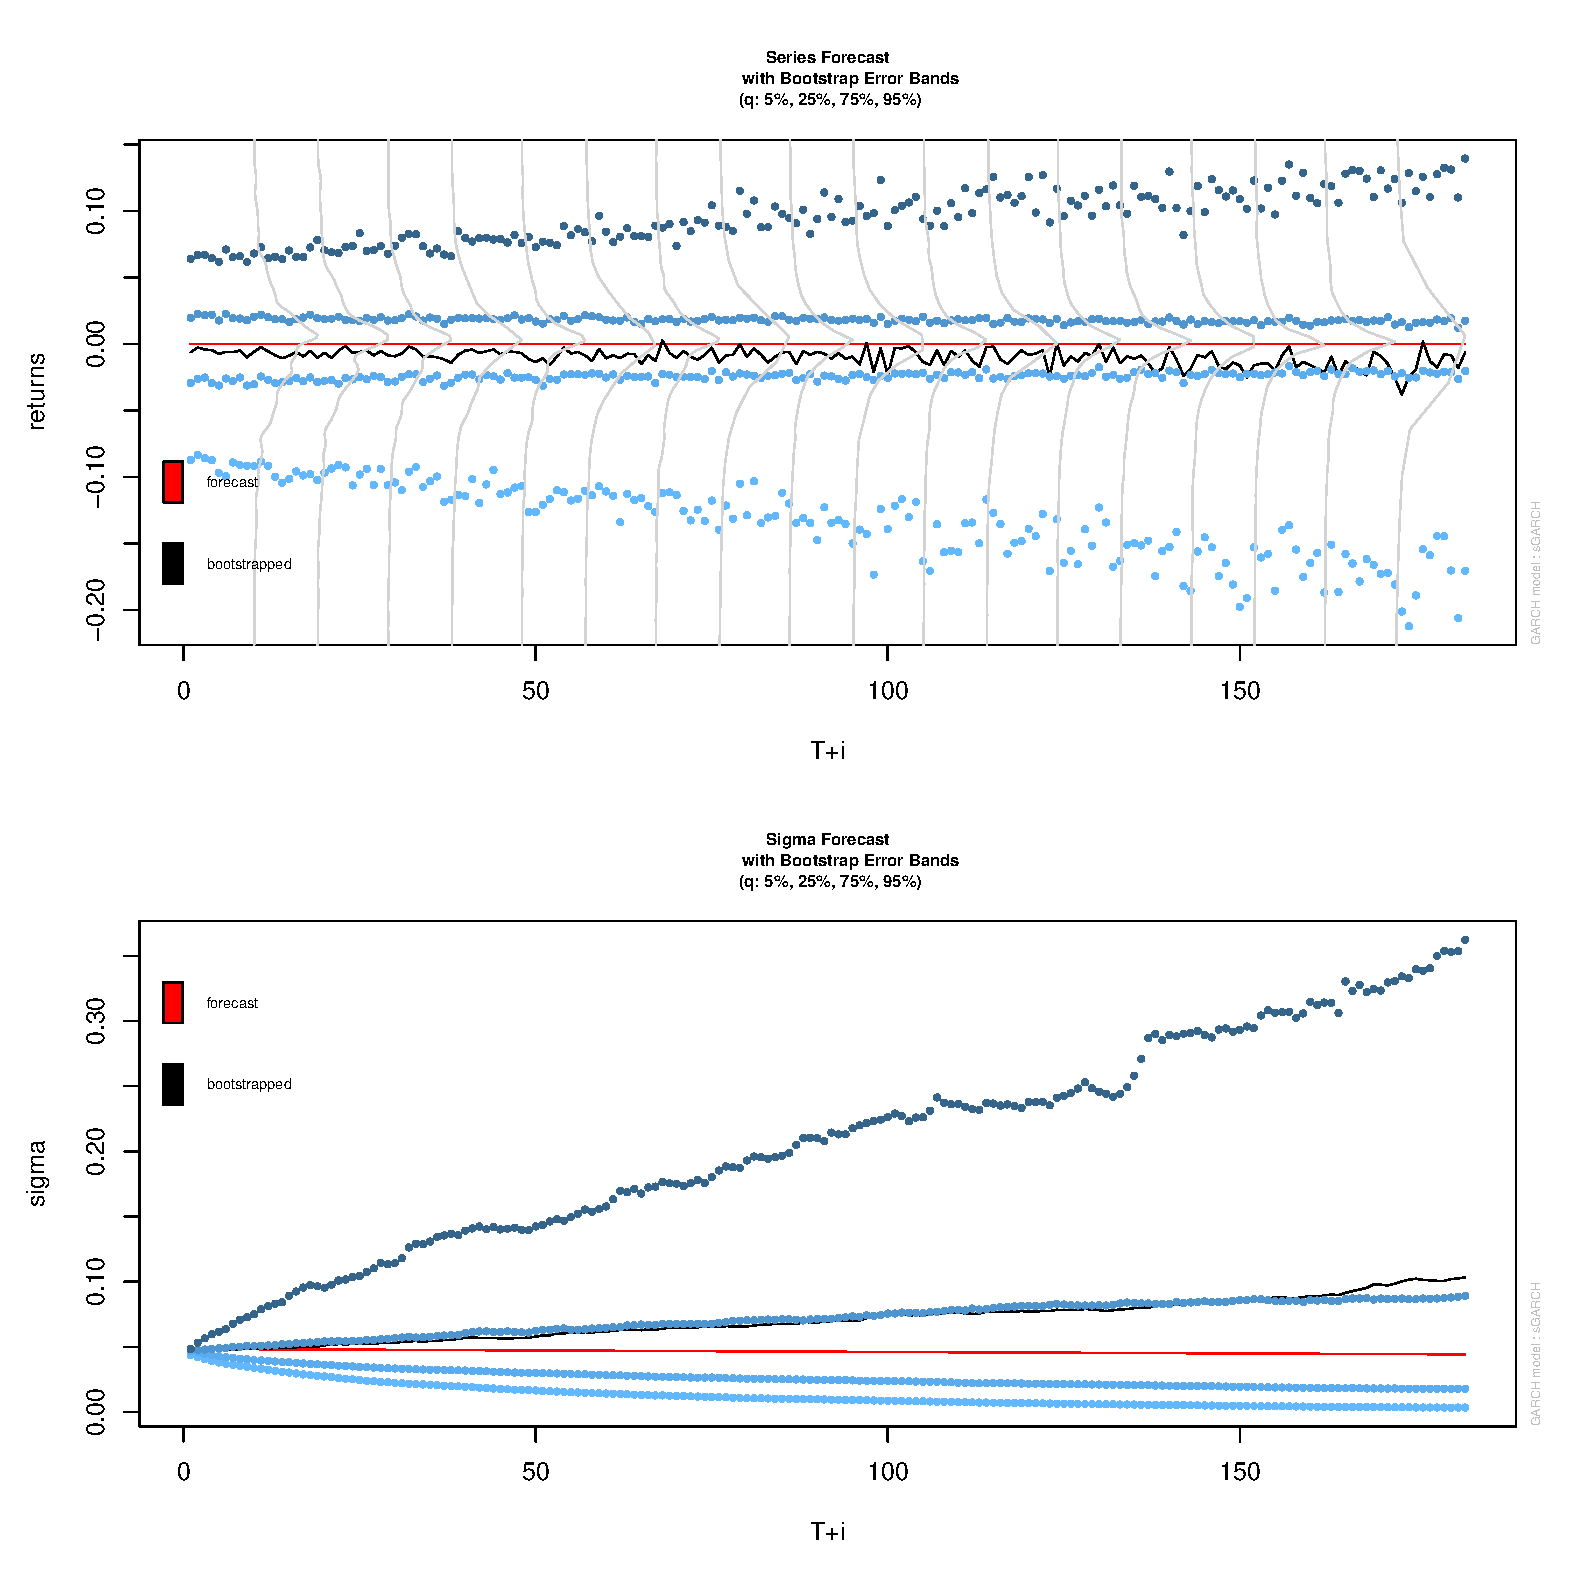
\includegraphics[width=.9\linewidth,height=.65\linewidth]{boot_cast_recent}\\
\caption{Bootstrap forecasting for fitted models. Top two plots are forecasted time-series and residual standard error for all data; bottom two plots are for recent (past-year) data. Note the increased volatility with time in both models.}
\label{fig:cast}
\end{center}
\end{figure}

\clearpage

\newpage
\bibliography{citations}
\bibliographystyle{plain}

\vspace{5cm}


\textbf{Group member contributions.} This project was the culmination of our discussions and work together, but we focused on different aspects. August Jensen researched and wrote about the GARCH model theory. Kurt Ehlert wrote the R code for fitting the ARMA-GARCH models and wrote up the model fitting analysis. Bi Cheng Wu constibuted the section on bootstrapping and forecasting.

\newpage

\appendix
\begin{center}
{\Large {\bf Appendix: \R\ code}}
\end{center}

\section{Model Fitting:}
Note: There is some output interspersed in the R code below.
% INSERT R CODE HERE, 10 point font
{\footnotesize
\begin{verbatim}
library(XLConnect)
library(xts)
library(rugarch)
library(TSA)
library(aTSA)

colTypes = c("DATETIME", rep("NUMERIC", 7))
raw_data = readWorksheetFromFile("/Bitcoin_daily_data.xlsx",sheet="Sheet1", header=T,
                                 dateTimeFormat="%m/%d/%Y", colTypes=colTypes, 
                                 forceConversion=TRUE)
data = xts(raw_data[,c("Open", "High", "Low", "Close")], order.by=raw_data$Date)

log_ret = tail(diff(log(data$Close), lag=1), n=-1)

recent_data = tail(data, n=1*365)
recent_log_ret = tail(diff(log(recent_data$Close), lag=1), n=-1)

plot(log_ret, main="Log ret.", lwd=0.5, yaxis.right=FALSE)
plot(recent_log_ret, main="Log ret.", lwd=0.5, yaxis.right=FALSE)

adf.test(coredata(log_ret))

Augmented Dickey-Fuller Test 
alternative: stationary 
 
Type 1: no drift no trend 
     lag   ADF p.value
[1,]   0 -44.9    0.01
[2,]   1 -32.5    0.01
[3,]   2 -26.4    0.01
[4,]   3 -22.3    0.01
[5,]   4 -19.0    0.01
[6,]   5 -16.1    0.01
[7,]   6 -15.3    0.01
[8,]   7 -14.7    0.01
Type 2: with drift no trend 
     lag   ADF p.value
[1,]   0 -44.9    0.01
[2,]   1 -32.5    0.01
[3,]   2 -26.5    0.01
[4,]   3 -22.4    0.01
[5,]   4 -19.1    0.01
[6,]   5 -16.2    0.01
[7,]   6 -15.4    0.01
[8,]   7 -14.8    0.01
Type 3: with drift and trend 
     lag   ADF p.value
[1,]   0 -44.9    0.01
[2,]   1 -32.5    0.01
[3,]   2 -26.5    0.01
[4,]   3 -22.4    0.01
[5,]   4 -19.1    0.01
[6,]   5 -16.2    0.01
[7,]   6 -15.4    0.01
[8,]   7 -14.8    0.01

acf(coredata(log_ret), lag.max=60, main="ACF of the log returns")
pacf(coredata(log_ret), lag.max=60, main="PACF of the log returns")
acf(coredata(log_ret)^2, lag.max=60, main="ACF of the squared log returns")
eacf(coredata(log_ret))

AR/MA
  0 1 2 3 4 5 6 7 8 9 10 11 12 13
0 o o o o x x o o o x x  o  o  o 
1 x o o o o x x o o o x  o  o  o 
2 o x o o o x o o o o x  o  o  o 
3 o x o o o x o o o o x  o  o  o 
4 x x o x o x o o o o x  o  o  o 
5 x x x x x o o o o o o  o  o  o 
6 x x x x x o o o o o o  o  o  o 
7 x x o x x x x o o o o  o  o  o 

fit = arima(log_ret, order=c(0,0,11))
tsdiag(fit)

fixed = c(0, 0, 0, 0, NA, NA, 0, 0, 0, NA, NA, 0)
fit = arima(x = log_ret, order = c(0, 0, 11), fixed = fixed)
(1-pnorm(abs(fit$coef[c(5, 6, 10, 11)])/sqrt(diag(fit$var.coef))))*2

        ma5         ma6        ma10        ma11 
0.027790261 0.004886633 0.011759164 0.009639468 

Box.test(residuals(fit),type="Ljung-Box", lag=30, fitdf=4)

data:  residuals(fit)
X-squared = 46.898, df = 26, p-value = 0.007227

mean.model=list(armaOrder=c(0,11))
spec = ugarchspec(variance.model = list(model = 'sGARCH', garchOrder = c(2, 2)),
                  mean.model=mean.model, distribution.model="std")
setfixed(spec) <- list(ma1=0, ma2=0, ma3=0, ma4=0,ma5=0, ma7=0, ma8=0, ma9=0,
                       ma10=0, ma11=0, alpha2=0, beta2=0, omega=0)
fit = ugarchfit(spec, log_ret, solver="hybrid")
plot(fit, which="all")

mean.model=list(armaOrder=c(0,0))
spec = ugarchspec(variance.model = list(model = 'sGARCH', garchOrder = c(1, 1)), 
                  mean.model=mean.model, distribution.model="sstd", 
                  fixed.pars=list(mu=0, omega=0))
fit = ugarchfit(spec, recent_log_ret, solver="hybrid")
plot(fit, which="all")

mean.model=list(armaOrder=c(0,0))
spec = ugarchspec(variance.model = list(model = 'eGARCH', garchOrder = c(1,1)), 
                  mean.model=mean.model, distribution.model="std", 
                  fixed.pars=list(omega=0, mu=0))
fit = ugarchfit(spec, recent_log_ret, solver="hybrid")
plot(fit, lwd=0.5, which="all")
\end{verbatim}}

\section{Model Evaluation:}

{\footnotesize
\begin{verbatim}
library(xts)
library(rugarch)
load("Bitcoin.Rdata")

recent_data = tail(data, n=1*365)
recent_log_ret = tail(diff(log(recent_data$Close), lag=1), n=-1)

mean.model=list(armaOrder=c(0,0))
spec = ugarchspec(variance.model = list(model = 'sGARCH', garchOrder = c(1, 1)),
                  mean.model=mean.model, distribution.model="std",
                  fixed.pars=list(mu=0,omega=0))
fit = ugarchfit(spec, recent_log_ret, solver="hybrid")

spec <- getspec(fit)
setfixed(spec) <- as.list(coef(fit))

cl = makeCluster(2,type="FORK")
bootp = ugarchboot(fit,method="Full",n.ahead=182,n.bootpred=1000,
                   cluster=cl,verbose=T)
stopCluster(cl)
save(bootp,file="bootp_recent.Rdata")
plot(bootp,which=1)
plot(bootp,which='all')
\end{verbatim}
}
\end{document}